\chapter{Ultrasonido}
\subsection{Objetivo}
Implementar un circuito capaz de hacer mediciones de distancia con un sensor ultrasonico HC-SR04 (diseñado para ser usado en Arduino) sin el uso de ningún tipo de logica programable.
\subsection{Analisis}
Para poder empezar con el proceso de diseño se analizaron todas las etapas por las que deberian viajar las señales con el fin de realizar lo pedido.
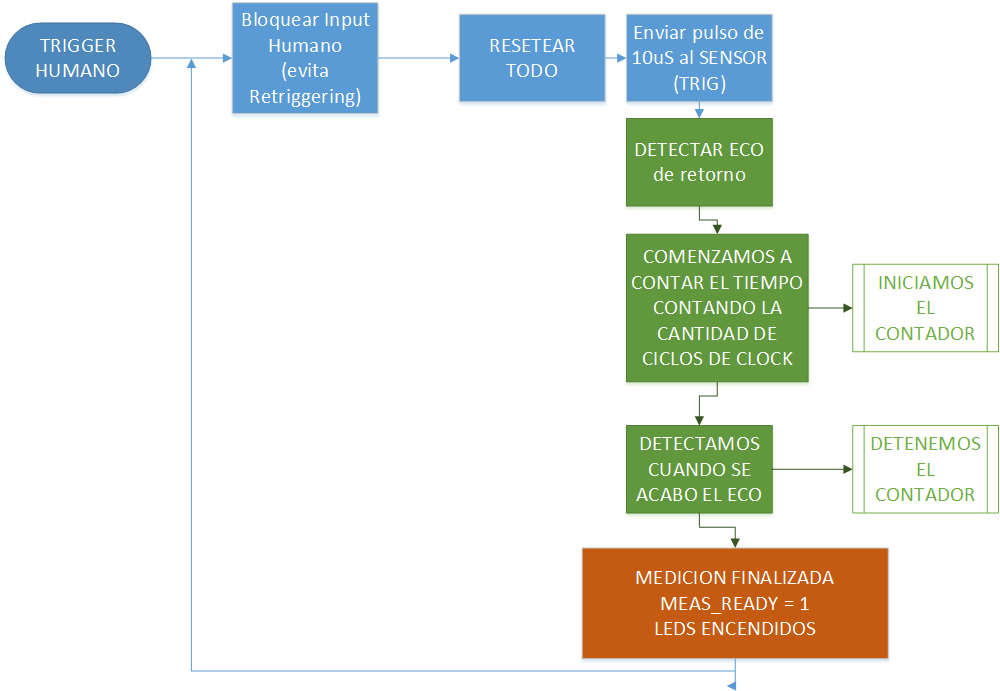
\includegraphics[scale=1]{../8-UltraSound/Driagrama-de-Flujo.png}
Dado que estamos trabajando con compuertas logicas fue bastante razonable pensar que en algún punto del diseño
